\chapterA{Hito 3 - Requisitos}

\section{Personas}

Tendremos dos personas, Marta (ver foto \ref{fig:fotoMarta}) e Isabel (ver foto \ref{fig:fotoIsaP}) \\

Para configurar estas personas, hemos utilizado un formato en el que vamos a dar en primer lugar la información general de la persona 
(edad, sexo, estudios y gustos). Posteriormente vamos a poner una foto de la persona (generada por una inteligencia artificial) y por último 
una descripción más elaborada de la persona, conteniendo la gran mayoría de los factoides e ideas expresadas en los esqueletos de las personas. 
Para poder destacar estas ideas, las hemos puesto en cursiva. \\

La estructura que van a tener las distintas personas va a seguir la siguiente configuración (ver figura \ref{fig:estructura-personas}) con los contenidos que hemos mecionado anteriormente.
\begin{figure}[h]
    \centering
    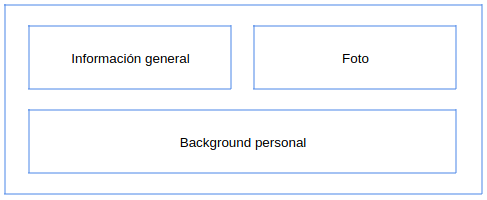
\includegraphics[width=0.5\textwidth]{Imagenes/Personas/Plantilla personas.png}
    \caption{Estructura de las personas}
    \label{fig:estructura-personas}
\end{figure}

\subsubsection{Marta González Torres}

\begin{minipage}{0.4\textwidth}
    \textbf{Información general} \\

    Edad: \textit{23 años} \\
    Sexo: Mujer \\
    Estudios: Ingeniería de Telecomunicaciones \\
    Gustos: Escuchar música e ir a conciertos cuando puede \\
\end{minipage}
\hfill
\begin{minipage}{0.4\textwidth}
    \centering
    
\includegraphics[width=0.5\textwidth]{Imagenes/Personas/Marta.jpg}
    \label{fig:fotoMarta}
    \captionof{figure}{Fotografía de Marta}
\end{minipage}

\textbf{Background personal} \\

Marta no puede salir de su casa sin los auriculares. Para ella la música es una gran parte
de su vida, y todas las mañanas, en la parada del bus, \textit{se prepara un playlist personalizada
en Spotify} para el itinerario hasta la Universidad. \textit{Vive en Fuenlabrada}, por lo que tiene
una ruta de una hora hasta que llega a Madrid, \textit{donde va a clase en la UCM}. \\ 

A Marta sobre todo le gusta la música italiana, ya que en el 2020 se fue de Erasmus a Turín y se
enamoró tanto de su cultura como de su música. Su cantante favorita es Francesca Michielin, así que
cuando hace gira intenta ir a algún concierto suyo en una \textit{ciudad italiana en la que no haya
estado}. De esta manera, puede conocer más la cultura italiana que tanto le gusta y sus diferenciados
a lo largo del país. \\

Se da la casualidad de que a su hermano Julián también le gusta mucho Francesca, así que en varias
ocasiones \textit{han ido ellos de viaje junto a sus padres} Carlos y Elena, los cuáles se van a
cenar juntos mientras sus hijos están en el concierto. \textit{Esto no lo hacen muy a menudo} debido
a que solo van cuando hay un concierto en alguna ciudad que les resulte interesante a toda la familia.
Normalmente se encarga ella de hacer la reserva tanto de los vuelos, \textit{para lo que usa
SkyScanner, como del alojamiento, utilizando AirBnB en este caso}. Esto se le hace a veces complicado
ya que quieren ir a varios sitios y tiene que cuadrar los horarios de todo. Por este motivo prefiere usar la 
aplicación web de las compañías, ya que así puede tener varias pestañas abiertas en las que visualiza toda
la información a la vez. \\

Con respecto al tema universitario, a Marta se le está haciendo cuesta arriba. Se metió inicialmente
en telecomunicaciones porque \textit{se le daban bien las matemáticas y la tecnología}, pero la
carrera no fue lo esperado. A pesar de las dificultades, la carrera le gusta y querría terminarla,
ya que este será en principio su último año. Pero estos problemas la agobian bastante, y para
distraerse le gusta mucho \textit{ir a festivales de música por España}. Suele ir todos los años
al festival Starlite, pues Pablo, el novio de su hermano y con el que mantiene muy buena relación,
es de Marbella, y se puede quedar algunos días en la playa aprovechando el viaje. Pero a pesar de
que no tiene que pagar gastos de alojamiento, el evento musical es bastante caro (ya que va varios
días), por lo que \textit{intenta ahorrar lo máximo posible en el viaje}. Para eso usa comparadores
de viaje como Omio, además de revisar las páginas de aerolíneas como \textit{RyanAir}, ya que a veces son
incluso más baratas que un vuelo o un tren.

\subsubsection{Isabel García Rodríguez}
\begin{minipage}{0.4\textwidth}
    \textbf{Información general} \\

    Edad: \textit{30 años} \\
    Sexo: Mujer \\
    Estudios: Psicología \\
    Gustos: Pintura y participar en grupos de apoyo para personas con discapacidad. \\
\end{minipage}
\hfill
\begin{minipage}{0.4\textwidth}
    \centering
    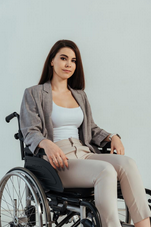
\includegraphics[width=0.5\textwidth]{Imagenes/Personas/Isabel.png}
    \label{fig:fotoIsaP}
    \captionof{figure}{Fotografía de Isabel}
\end{minipage}

\textbf{Background personal} \\

Isabel es una psicóloga comprometida con la mejora de la calidad de vida de las personas con discapacidad. \textit{Tiene una 
discapacidad física desde su nacimiento} que afecta su movilidad y requiere el uso de una silla de ruedas. Actualmente
\textit{vive en una pequeña urbanización a las afueras de Barcelona}. \\

Su familia vive en un pequeño pueblo de Huesca, por lo que \textit{siempre que puede se desplaza para verlos}. Muchas veces 
tiene el problema de la falta de autobuses que conectan con el pueblo, por lo que \textit{utiliza Omio, que realiza el trayecto
por ella, indicándole los transbordos que tiene que realizar y facilitándole la ayuda que necesita en todo momento}. \\

Ha asistido a varios cursos y conferencias relacionados con la psicología y la discapacidad, lo que la ha llevado a 
\textit{planear viajes a diferentes ciudades para participar en eventos}. Utiliza comparadores de viaje para encontrar opciones 
que se adapten a sus necesidades específicas, como hoteles con habitaciones adaptadas y \textit{vuelos con asistencia en el 
aeropuerto}. \textit{Algunos de los comparadores que usa no tienen opción de solicitar ayuda en caso de que tengas dudas, por lo que si
tiene algún problema no puede contactar con nadie}. Antes de realizar la reserva, ella sabe las distintas compañías y empresas que te lo suelen proporcionar. \\

Aparte de su trabajo, Isabel es una apasionada de la pintura y trata de visitar galerías y estudios de artistas en cada 
destino que visita. Isabel también es miembro activo de grupos de apoyo para personas con discapacidad en su ciudad. \textit{Allí 
es donde comparte experiencias y ofrece apoyo a otros miembros, por ejemplo a los jóvenes con discapacidad, para fomentar 
su independencia y autoestima}. Viaja a menudo con su mejor amiga, Carmen, quien la ha apoyado en su viaje de empoderamiento 
y ha aprendido mucho sobre la discapacidad en el proceso también.

\subsection{Tipos de personas}
\begin{itemize}
    \item \textbf{Persona Primaria} - \textit{Marta González Torres (Viajero que usa comparadores de viajes)} $\rightarrow$ Representa al tipo de usuario consumidor de comparadores de viajes. Se tratan de usuarios que utilizan activamente las funcionalidades de los comparadores con el objetivo de ahorrar lo máximo posible en los transportes para sus viajes.
    \item \textbf{Persona Secundaria} - \textit{Isabel García Rodríguez (Viajero con discapacidad)} $\rightarrow$ Representa al tipo de usuario consumidor o no consumidor de comparadores de viajes que tienen una necesidad añadida o distinta al resto de usuarios. 
    Generalmente usuarios que aparte de la interfaz ya creada necesitaran de una pequeña adaptación visual o sensorial para poder sacar el máximo provecho a la aplicación. En el caso de Isabel necesitaría un apoyo extra debido a su discapacidad que presenta, ya que sus viajes esterían mucho más condicionados que los de Marta.
\end{itemize}

\section{Fase de Requisitos}
La siguiente fase que vamos a abordar en el proceso de Diseño Guiado por Objetivos (DGO) es la fase de requisitos. En esta fase, vamos a tomar como punto de partida las personas que generamos en el hito anterior. A partir de ellas, vamos a estudiarlas en profundidad para obtener soluciones de diseño que satisfagan sus necesidades. Para ello, el proceso que vamos a seguir para definir los requisitos de las personas va a ser el método propuesto por Cooper, que consta de cuatro etapas diferenciadas:
\begin{enumerate}
	\item \textbf{Enunciado de problemas y visiones} $\rightarrow$ vamos a estudiar en detalle la información contenida en las personas que hemos desarrollado, 
    de modo que a partir de ellas vamos a intentar identificar los problemas que tienen y aportar cómo vamos a plantear una solución para este problema.
    \item \textbf{Identificación de las expectativas de las personas} $\rightarrow$ en esta segunda etapa, se va a tomar como punto de partida las distintas personas
    y para cada una de ellas vamos a analizar sus pensamientos, deseos, comportamientos y conocimientos que la persona va a tener en el ámbito de la aplicación.
    \item \textbf{Construcción de los escenarios de contexto} $\rightarrow$ en este apartado, van a redactarse para cada una de las personas que se han identificado, un
    escenario de contexto, que ponga en situación a la persona, persiguiendo un objetivo y describiendo el proceso que sigue para ello.
    \item \textbf{Identificaión de requisitos} $\rightarrow$ se trata de la fase final de este hito. En este apartado van a aparecer fusionadas todos los requisitos de
    las distintas personas que hemos ejemplificado, determinando cuáles son las necesidades que tienen y cuál va a ser el medio que necesitan para que puedan ser
    satisfechas estas necesidades en nuestra aplicación.
\end{enumerate}

\section{Planificación del hito}
Para poder planificar este hito correctamente, hemos identificado en una Hoja de cálculo (ver figura \ref{fig:planif-hito3}) las distintas tareas que tenemos que 
realizar, junto al intervalo de fechas en el que se encuentra prevista su realización y el / los responsables de dicha tarea.
\begin{figure}[H]
    \centering 
    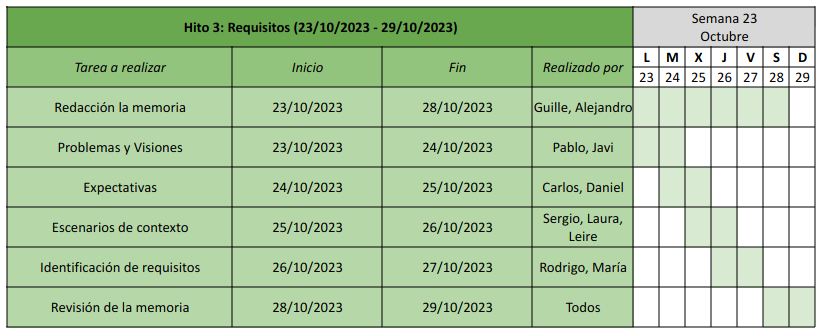
\includegraphics[width=0.5\textwidth]{./Imagenes/Planificaciones/Planif-hito3.png}
    \caption{Planificación Hito 3}
    \label{fig:planif-hito3}
\end{figure}

\section{Enunciado de problemas y visiones}

Tras evaluar las personas obtenidas y sus objetivos, procedemos a ver los distintos problemas que se nos plantean y la visión de nuestra aplicación para resolver cada uno de ellos. Con estos problemas y visiones podremos focalizar las distintas partes y funcionalidades de la aplicación final.

\begin{problema}

    Hay personas que no tienen un gran poder adquisitivo y tienen que ajustar su presupuesto para organizar el viaje 

    {\centering
    \begin{vision} \justifying \noindent
        Nuestra aplicación ofrecerá los viajes más baratos al comienzo de la búsqueda cuando el usuario lo solicite dentro de unas fechas y una serie de filtros.

    \end{vision}}
\end{problema}

\vspace{0.5cm}

\begin{problema}
    No conocer de antemano toda la información y/o ventajas de las que se disponga.

    {\centering
    \begin{vision}\justifying \noindent
        Nuestra aplicación contará con toda la información detallada así como con un apartado en el que estarán especificados los servicios que ofrecemos. También contaremos con una serie de recursos para que los usuarios puedan comunicarse con el servicio al cliente.
    \end{vision}}
\end{problema}


\vspace{0.5cm}

\begin{problema}

    Numerosas aplicaciones web o móviles no están adaptadas a las diferentes discapacidades que puedan poseer los usuarios
    
    {\centering
    \begin{vision}\justifying \noindent
        Nuestra aplicación contará con el Nivel Triple-A de Conformidad con las Directrices de Accesibilidad para el Contenido Web 1.0 (WCAG 1.0) para ser accesible para todo tipo de usuarios.
    \end{vision}}
\end{problema}


\vspace{0.5cm}

\begin{problema}

    Las personas con discapacidad física muchas veces deben hacer un esfuerzo extra a la hora de saber si pueden reservar un viaje en algún transporte ya que no viene de forma clara que exista una adaptabilidad para estas personas.

    {\centering
    \begin{vision}\justifying \noindent
        Nuestra aplicación contará con toda la información sobre las diferentes discapacidades y cómo poder ayudar a los distintos usuarios así como nuestros trabajadores poseerán la información necesaria para poder contactar con las diferentes empresas de transporte y poder mediar entre el usuario y la empresa para poder viajar cómodo y seguro sin preocupaciones.
    \end{vision}}
\end{problema}
    
\newpage

\begin{problema}

    Las aplicaciones móviles son menos intuitivas que las webs porque ofrecen menos información y está todo más compacto.

    {\centering
    \begin{vision}\justifying \noindent
        Nuestra aplicación va a ofrecer la información justa y necesaria, sacaremos una versión “Alpha” para poder aprender de ella y mejorarla a través del uso.

    \end{vision}}
\end{problema}
    


\section{Identificación de las expectativas de las personas}
En la siguiente fase del proceso de identificación  de requisitos, se ha realizado una identificación de las distintas expectativas de las personas, exponiendo para cada una 
de ellas su pensamiento de qué es lo que esperan de la aplicación, teniendo en cuenta los distintos problemas que tienen que afrontar el el proceso.

\subsection{Expectativas de Marta}
A Marta le encanta la música e ir a los conciertos de su cantante favorita, Francesca Michielin. Así que cuando hace gira intenta ir a algún concierto en alguna 
ciudad italiana, en la que no ha estado, con su hermano y sus padres, espera que la aplicación le permita hacer reservas de vuelos. A Marta le resulta más cómodo 
usar aplicaciones web de escritorio por lo que espera poder hacer las reservas a través de la web en su ordenador. \\

A Marta también le gusta ir a festivales de música por España para distraerse de la universidad, como los festivales son muy caros, espera que la aplicación 
le permita encontrar las opciones más baratas para ajustarse lo máximo posible a su presupuesto comparando múltiples opciones de transporte y precios.


\subsection{Expectativas de Isabel}
Isabel ha asistido a cursos y conferencias y ha tenido que viajar para ir a ellos en distintas ciudades, como tiene una discapacidad espera que la aplicación 
le permita encontrar opciones que se adapten a sus necesidades, como asistente de vuelo. Isabel ha tenido que contactar alguna vez con el servicio del 
aeropuerto para conocer los servicios que ofrecen, por lo que espera que la aplicación incluyese esta información y la posibilidad de contratarlo desde la misma.

\section{Construcción de los escenarios de contexto}
Un escenario es una situación narrativa, una historia concreta y realista que involucra a una persona y narra de manera detallada cómo persigue un objetivo y
finalmente logra satisfacer dicho objetivo, describiendo el proceso que ha seguido para ello. Cada uno de estos escenarios va a describir cómo se va a comportar
el usuario (en este caso la persona) en el contexto de la aplicación, definiendo en todo momento qué es lo que tiene que realizar para poder afrontar un problema
concreto.
\subsection{Escenarios de contexto de Marta}
\begin{itemize}
    \item \textbf{Concierto en la ciudad equivocada} $\rightarrow$ Hace unos días Francesca anunció una gira por Italia. Marta y su
    hermano no se pueden perder esto, por lo que saca la aplicación y selecciona como destino todas las ciudades de
    la gira junto a las fechas. Los dos se ponen a mirar a la vez, cada uno en su portátil, y ven que el vuelo más
    barato es a Milán. !`Solo 15\euro  cada uno! Pero desgraciadamente, el día que sale ese vuelo, Francesca canta en Turín.
    Cuando estaban a punto de descartarlo, Marta se acordó de cuando estuvo de Erasmus que Turín está a apenas 2 horas
    en tren de Milán. Como toda la información de la app es fácilmente visible, pudo ver a qué hora llegaba y en qué
    aeropuerto, para así buscar en la misma app un tren que fuese a Turín, fijándose tanto de la distancia a la que estaba el la estación como de los horarios, para poder llegar sin problemas pero que también le diese tiempo a llegar al concierto. Justo cuando ya las habían encontrado e iban a pagar para terminar con la compra de los billetes después de una larga planificación para poder cumplir con lo que se habían propuesto, se les va el Internet. Cuando vuelve el Internet tienen aún todo guardado y finalmente, han podido comprar los billetes aliviados.
    
    \item \textbf{Cambio de planes por motivo económico} $\rightarrow$ Es época de exámenes y Marta está muy agobiada.
    No está muy segura de si ha aprobado las asignaturas que lleva o de cómo le van a salir las que le faltan. Su amiga
    Pili, viendo el agobio de Marta, le ha dicho de irse a Ibiza de fiesta el finde posterior a los exámenes, de esta
    manera tiene mayor aliciente para continuar con las semanas que le quedan. A Marta le encantó la idea, así que
    enseguida sacó la app y buscó vuelos ese finde a Ibiza. Desgraciadamente, estaba un poco justa de dinero porque no
    está trabajando por el momento, y los precios que tenía el vuelo eran demasiado caros para su bolsillo. Afortunadamente,
    pudo ver en la aplicación que el mismo día salía un vuelo a Palma de Mallorca, y les costaba la ida y vuelta 50€
    menos. A Pili le pareció bien cambiar el plan de fiesta a un plan de playa, así que compraron los billetes, deseosas
    de que acaben.
\end{itemize}
\subsection{Escenarios de contexto de Isabel}
\begin{itemize}
    \item \textbf{Viaje inesperado} $\rightarrow$ Es lunes e Isabel va a tomar un café con sus compañeros de trabajo, como de costumbre. Mientras espera a 
    que le traigan el desayuno, su móvil empieza a sonar y al mirar quién la está llamando, ve que es su jefe. Éste le dice que el miércoles hay una conferencia 
    para la inclusión de niños con discapacidad y que la mujer que iba a dar la ponencia ha tenido un imprevisto y no podrá darla, por lo que le ofrece a Isabel 
    sustituirla.\\
    Aunque es muy precipitado, Isabel acepta y empieza a buscar transporte. Abre la aplicación y selecciona en el apartado filtros, persona con discapacidad 
    física, y ve el abanico de posibilidades de vuelos accesibles para ella. Al ser un viaje que no tenía previsto, su objetivo es ahorrar el máximo dinero 
    posible, por lo escoge el más barato. Contenta con su compra, se va a casa a preparar la maleta.
    \item \textbf{Problemas de gestión} $\rightarrow$ Carmen e Isabel llevan varios meses intentando ir a la exposición de arte de un artista emergente que les 
    gusta mucho. En Barcelona las entradas se agotaron a los pocos minutos de salir, por lo que no consiguieron. Ahora ha vuelto con otra exposición, pero esta 
    vez en Madrid. \\
    Como Carmen e Isabel no se la quieren perder, han decidido que viajarán a Madrid un par de días. La exposición estará un mes entero, pero no saben qué días irán.
    Isabel abre la aplicación y busca los trenes de Renfe en el mes completo que más se ajustan a sus horarios. Eligen esta compañía ya que Carmen tiene 
    descuentos. Cuando ya ha comprado los billetes, espera un período de tiempo para recibirlos en su correo, pero no llegan. Desde la aplicación se pone en contacto 
    con el servicio al cliente, que le dice que están teniendo problemas con la gestión de los billetes y que se lo resuelven de forma manual en pocos minutos. Y así 
    fue, instantes después, Isabel ya tenía sus billetes.
\end{itemize}

\section{Identificación de requisitos}
Tras hacer un estudio de problemas, expectativas y escenarios de contexto, la última etapa de esta fase de requisitos. En esta fase se van a exponer claramente las 
necesidades de la persona para satisfacer sus objetivos. Dicho de otro modo, se trata de definir qué es lo que va a hacer nuestra aplicación (pero sin entrar en
detalle en cómo lo va a hacer). Los requisitos que hemos identificado son los siguientes:
\begin{itemize}
    \item Buscar (\textit{\underline{acción}}) transportes disponibles (\textit{\underline{objeto}}) a las ciudades designadas (\textit{\underline{contexto}}).
    \item Filtrar (\textit{\underline{acción}}) tipo de transporte (\textit{\underline{objeto}}) según preferencia/necesidad (\textit{\underline{contexto}}).
    \item Seleccionar (\textit{\underline{acción}}) fechas concretas o un intervalo de tiempo (\textit{\underline{objeto}}) para la búsqueda del transporte (\textit{\underline{contexto}}).
    \item Comparar (\textit{\underline{acción}}) precios (\textit{\underline{objeto}}) de los diferentes transportes a la ciudad designada (\textit{\underline{contexto}}).
    \item Ordenar (\textit{\underline{acción}}) los transportes por precios y/o fechas (\textit{\underline{objeto}}) según las necesidades, para agilizar la búsqueda (\textit{\underline{contexto}}).
    \item Reservar (\textit{\underline{acción}}) billetes (\textit{\underline{objeto}}) de los transportes deseados (\textit{\underline{contexto}}).
    \item Seleccionar (\textit{\underline{acción}}) tipo de transporte (\textit{\underline{objeto}}) según preferencias y/o precio (\textit{\underline{contexto}}).
    \item Ofrecer (\textit{\underline{acción}}) información sobre horarios de transporte (\textit{\underline{objeto}}) al realizar la búsqueda (\textit{\underline{contexto}}).
    \item Ofrecer (\textit{\underline{acción}}) información de los asientos disponibles (\textit{\underline{objeto}}) del vehículo seleccionado (\textit{\underline{contexto}}).
    \item Seleccionar (\textit{\underline{acción}}) asientos (\textit{\underline{objeto}}) una vez elegido el transporte (\textit{\underline{contexto}}).
    \item Ofrecer (\textit{\underline{acción}}) diferentes rutas (\textit{\underline{objeto}}) cuando seleccionas una serie de destinos (\textit{\underline{contexto}}).
    \item Ofrecer (\textit{\underline{acción}}) servicios disponibles en el transporte (\textit{\underline{objeto}}) cuando seleccionas un transporte en concreto (\textit{\underline{contexto}}).
    \item Indicar (\textit{\underline{acción}}) la zona de recogida, origen y destino (\textit{\underline{objeto}}) del vehículo a lo largo del trayecto (\textit{\underline{contexto}}).
    \item Buscar (\textit{\underline{acción}}) transportes disponibles (\textit{\underline{objeto}}) para un viaje inmediato o de última hora (\textit{\underline{contexto}}).
    \item Filtrar (\textit{\underline{acción}}) opciones de transporte (\textit{\underline{objeto}}) específicas para personas con discapacidad física (\textit{\underline{contexto}}).
    \item Mostrar (\textit{\underline{acción}}) información detallada (\textit{\underline{objeto}}) sobre la accesibilidad de los transportes disponibles (\textit{\underline{contexto}}).
    \item Permitir (\textit{\underline{acción}}) la compra de billetes de transporte (\textit{\underline{objeto}}) de manera rápida y sencilla para viajes inesperados (\textit{\underline{contexto}}).
    \item Ofrecer (\textit{\underline{acción}}) descuentos y promociones de transporte (\textit{\underline{objeto}}) para viajes en pareja o con compañeros(\textit{\underline{contexto}}).
    \item Facilitar (\textit{\underline{acción}}) la compra de billetes (\textit{\underline{objeto}}) en línea y proporcionar una entrega eficiente de los mismos (\textit{\underline{contexto}}).
    \item Ofrecer (\textit{\underline{acción}}) soporte al cliente (\textit{\underline{objeto}}) para resolver problemas de gestión de billetes de manera rápida y eficaz (\textit{\underline{contexto}}).
\end{itemize}
